% Options for packages loaded elsewhere
\PassOptionsToPackage{unicode}{hyperref}
\PassOptionsToPackage{hyphens}{url}
%
\documentclass[
]{book}
\title{SEDSI 2022}
\author{Tobin Turner}
\date{2022-02-17}

\usepackage{amsmath,amssymb}
\usepackage{lmodern}
\usepackage{iftex}
\ifPDFTeX
  \usepackage[T1]{fontenc}
  \usepackage[utf8]{inputenc}
  \usepackage{textcomp} % provide euro and other symbols
\else % if luatex or xetex
  \usepackage{unicode-math}
  \defaultfontfeatures{Scale=MatchLowercase}
  \defaultfontfeatures[\rmfamily]{Ligatures=TeX,Scale=1}
\fi
% Use upquote if available, for straight quotes in verbatim environments
\IfFileExists{upquote.sty}{\usepackage{upquote}}{}
\IfFileExists{microtype.sty}{% use microtype if available
  \usepackage[]{microtype}
  \UseMicrotypeSet[protrusion]{basicmath} % disable protrusion for tt fonts
}{}
\makeatletter
\@ifundefined{KOMAClassName}{% if non-KOMA class
  \IfFileExists{parskip.sty}{%
    \usepackage{parskip}
  }{% else
    \setlength{\parindent}{0pt}
    \setlength{\parskip}{6pt plus 2pt minus 1pt}}
}{% if KOMA class
  \KOMAoptions{parskip=half}}
\makeatother
\usepackage{xcolor}
\IfFileExists{xurl.sty}{\usepackage{xurl}}{} % add URL line breaks if available
\IfFileExists{bookmark.sty}{\usepackage{bookmark}}{\usepackage{hyperref}}
\hypersetup{
  pdftitle={SEDSI 2022},
  pdfauthor={Tobin Turner},
  hidelinks,
  pdfcreator={LaTeX via pandoc}}
\urlstyle{same} % disable monospaced font for URLs
\usepackage{color}
\usepackage{fancyvrb}
\newcommand{\VerbBar}{|}
\newcommand{\VERB}{\Verb[commandchars=\\\{\}]}
\DefineVerbatimEnvironment{Highlighting}{Verbatim}{commandchars=\\\{\}}
% Add ',fontsize=\small' for more characters per line
\usepackage{framed}
\definecolor{shadecolor}{RGB}{248,248,248}
\newenvironment{Shaded}{\begin{snugshade}}{\end{snugshade}}
\newcommand{\AlertTok}[1]{\textcolor[rgb]{0.94,0.16,0.16}{#1}}
\newcommand{\AnnotationTok}[1]{\textcolor[rgb]{0.56,0.35,0.01}{\textbf{\textit{#1}}}}
\newcommand{\AttributeTok}[1]{\textcolor[rgb]{0.77,0.63,0.00}{#1}}
\newcommand{\BaseNTok}[1]{\textcolor[rgb]{0.00,0.00,0.81}{#1}}
\newcommand{\BuiltInTok}[1]{#1}
\newcommand{\CharTok}[1]{\textcolor[rgb]{0.31,0.60,0.02}{#1}}
\newcommand{\CommentTok}[1]{\textcolor[rgb]{0.56,0.35,0.01}{\textit{#1}}}
\newcommand{\CommentVarTok}[1]{\textcolor[rgb]{0.56,0.35,0.01}{\textbf{\textit{#1}}}}
\newcommand{\ConstantTok}[1]{\textcolor[rgb]{0.00,0.00,0.00}{#1}}
\newcommand{\ControlFlowTok}[1]{\textcolor[rgb]{0.13,0.29,0.53}{\textbf{#1}}}
\newcommand{\DataTypeTok}[1]{\textcolor[rgb]{0.13,0.29,0.53}{#1}}
\newcommand{\DecValTok}[1]{\textcolor[rgb]{0.00,0.00,0.81}{#1}}
\newcommand{\DocumentationTok}[1]{\textcolor[rgb]{0.56,0.35,0.01}{\textbf{\textit{#1}}}}
\newcommand{\ErrorTok}[1]{\textcolor[rgb]{0.64,0.00,0.00}{\textbf{#1}}}
\newcommand{\ExtensionTok}[1]{#1}
\newcommand{\FloatTok}[1]{\textcolor[rgb]{0.00,0.00,0.81}{#1}}
\newcommand{\FunctionTok}[1]{\textcolor[rgb]{0.00,0.00,0.00}{#1}}
\newcommand{\ImportTok}[1]{#1}
\newcommand{\InformationTok}[1]{\textcolor[rgb]{0.56,0.35,0.01}{\textbf{\textit{#1}}}}
\newcommand{\KeywordTok}[1]{\textcolor[rgb]{0.13,0.29,0.53}{\textbf{#1}}}
\newcommand{\NormalTok}[1]{#1}
\newcommand{\OperatorTok}[1]{\textcolor[rgb]{0.81,0.36,0.00}{\textbf{#1}}}
\newcommand{\OtherTok}[1]{\textcolor[rgb]{0.56,0.35,0.01}{#1}}
\newcommand{\PreprocessorTok}[1]{\textcolor[rgb]{0.56,0.35,0.01}{\textit{#1}}}
\newcommand{\RegionMarkerTok}[1]{#1}
\newcommand{\SpecialCharTok}[1]{\textcolor[rgb]{0.00,0.00,0.00}{#1}}
\newcommand{\SpecialStringTok}[1]{\textcolor[rgb]{0.31,0.60,0.02}{#1}}
\newcommand{\StringTok}[1]{\textcolor[rgb]{0.31,0.60,0.02}{#1}}
\newcommand{\VariableTok}[1]{\textcolor[rgb]{0.00,0.00,0.00}{#1}}
\newcommand{\VerbatimStringTok}[1]{\textcolor[rgb]{0.31,0.60,0.02}{#1}}
\newcommand{\WarningTok}[1]{\textcolor[rgb]{0.56,0.35,0.01}{\textbf{\textit{#1}}}}
\usepackage{longtable,booktabs,array}
\usepackage{calc} % for calculating minipage widths
% Correct order of tables after \paragraph or \subparagraph
\usepackage{etoolbox}
\makeatletter
\patchcmd\longtable{\par}{\if@noskipsec\mbox{}\fi\par}{}{}
\makeatother
% Allow footnotes in longtable head/foot
\IfFileExists{footnotehyper.sty}{\usepackage{footnotehyper}}{\usepackage{footnote}}
\makesavenoteenv{longtable}
\usepackage{graphicx}
\makeatletter
\def\maxwidth{\ifdim\Gin@nat@width>\linewidth\linewidth\else\Gin@nat@width\fi}
\def\maxheight{\ifdim\Gin@nat@height>\textheight\textheight\else\Gin@nat@height\fi}
\makeatother
% Scale images if necessary, so that they will not overflow the page
% margins by default, and it is still possible to overwrite the defaults
% using explicit options in \includegraphics[width, height, ...]{}
\setkeys{Gin}{width=\maxwidth,height=\maxheight,keepaspectratio}
% Set default figure placement to htbp
\makeatletter
\def\fps@figure{htbp}
\makeatother
\setlength{\emergencystretch}{3em} % prevent overfull lines
\providecommand{\tightlist}{%
  \setlength{\itemsep}{0pt}\setlength{\parskip}{0pt}}
\setcounter{secnumdepth}{5}
\usepackage{booktabs}
\ifLuaTeX
  \usepackage{selnolig}  % disable illegal ligatures
\fi
\usepackage[]{natbib}
\bibliographystyle{apalike}

\begin{document}
\maketitle

{
\setcounter{tocdepth}{1}
\tableofcontents
}
\hypertarget{sedsi-2022}{%
\chapter{SEDSI 2022}\label{sedsi-2022}}

\begin{center}
\includegraphics{_images/SEDSI} \end{center}

SEDSI Fun with Reproducible Analysis and RMarkdown

\hypertarget{motivation}{%
\chapter{Motivation}\label{motivation}}

A COVID Classroom

\begin{center}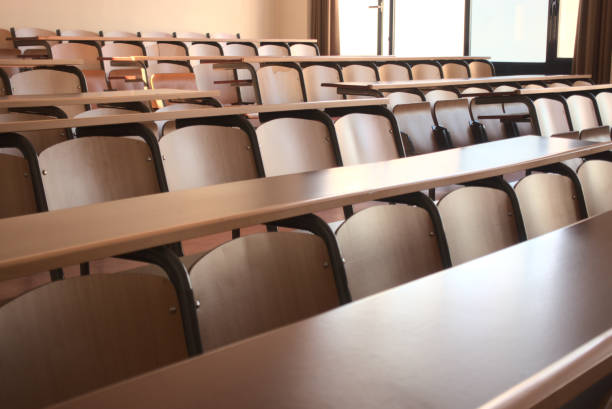
\includegraphics{_images/empty_class} \end{center}

A Learning Management System Nightmare

\begin{center}
\includegraphics{_images/brightspace} \end{center}

Concise, Precisely Organized, Frequently Revised Assignments and Schedules

\begin{longtable}[]{@{}ll@{}}
\toprule
Date & Topic \\
\midrule
\endhead
Wednesday, February 16, 2022 & SEDSI in Jacksonville \\
Thursday, February 17, 2022 & Present at 2:45 PM \\
Friday, February 18, 2022 & Celebrate a successful DASI Session \\
\bottomrule
\end{longtable}

\hypertarget{real-life-example}{%
\chapter{Real life example}\label{real-life-example}}

It's nice to know exactly what you did when your original data requires wrangling.

Conflicts and students honors\ldots{}

\begin{table}

\caption{\label{tab:unnamed-chunk-3}Some Actual Data We Considered}
\centering
\begin{tabular}[t]{l|r|r|r}
\hline
NAME & TOTAL.HOURS & PC.HOURS & ADMIT.TERM\\
\hline
Greer, Patrick Sterling & 3.0 & 3.0 & 201101\\
\hline
Greer, Patrick Sterling & 144.0 & 123.0 & 201101\\
\hline
Thompson, Charleston Hannah & 0.0 & 0.0 & 201201\\
\hline
Thompson, Charleston Hannah & 142.0 & 122.0 & 201201\\
\hline
Melvin, Victor Richard-Scorsese & 132.0 & 100.0 & 201202\\
\hline
Roberson, States Taylor & 126.0 & 99.0 & 201301\\
\hline
Allen, Kaylee Michelle & 125.0 & 68.0 & 201601\\
\hline
Phelps, Payton Elliott & 117.0 & 114.0 & 201701\\
\hline
Rowley, Ella Marie Dorothy & 121.0 & 121.0 & 201701\\
\hline
Smith, Michael Leston & 112.0 & 112.0 & 201701\\
\hline
Taylor, Darrell Tyrese & 78.0 & 78.0 & 201701\\
\hline
Wright, Alexandra Ruby & 116.0 & 116.0 & 201701\\
\hline
Adu, Tyler & 80.0 & 80.0 & 201801\\
\hline
Armell, James Richard & 90.0 & 87.0 & 201801\\
\hline
Bell, Carrie Abigail & 120.5 & 99.5 & 201801\\
\hline
Boyd, Jeremiah Quintin & 87.0 & 87.0 & 201801\\
\hline
Brinkley, Khalid Osmon & 74.0 & 74.0 & 201801\\
\hline
Campbell, Blakeney Herlong & 92.0 & 85.0 & 201801\\
\hline
Dearman, Clark Avant & 101.5 & 82.5 & 201801\\
\hline
Drake, John Chapman & 94.0 & 94.0 & 201801\\
\hline
\end{tabular}
\end{table}

\hypertarget{some-options}{%
\chapter{Some Options}\label{some-options}}

This is just a cool place to put stuff\footnote{Footnotes are always neat. And useful. Like this one!}.

Like a schedule, for example:

\hypertarget{spring-2022}{%
\section{Spring 2022}\label{spring-2022}}

\begin{longtable}[]{@{}ll@{}}
\toprule
Date & Topic \\
\midrule
\endhead
Monday, January 10, 2022 & R basics and install \\
Wednesday, January 12, 2022 & R basics and workflows \\
Friday, January 14, 2022 & QUIZ 1 \\
Monday, January 17, 2022 & MLK Holiday \\
Wednesday, January 19, 2022 & Objects, Vectors, and Arithmetic \\
Friday, January 21, 2022 & QUIZ 2 \\
Monday, January 24, 2022 & Summaries and Subscripting \\
\bottomrule
\end{longtable}

\hypertarget{or-a-figure}{%
\section{Or a figure}\label{or-a-figure}}

\includegraphics{01-intro_files/figure-latex/unnamed-chunk-4-1.pdf}

\hypertarget{or-an-equation}{%
\section{Or an Equation}\label{or-an-equation}}

Here is a \textbf{fun} equation for my SEDSI DASI friends:

\begin{equation} 
  f\left(k\right) = \binom{n}{k} p^k\left(1-p\right)^{n-k}
  \label{eq:binom}
\end{equation}

\hypertarget{or-a-table-of-something}{%
\section{Or a table of something}\label{or-a-table-of-something}}

\hypertarget{fun-example-table}{%
\subsection{Fun example table}\label{fun-example-table}}

\begin{table}

\caption{\label{tab:unnamed-chunk-5}A table of the first 10 rows of the mtcars data.}
\centering
\begin{tabular}[t]{lrrrrrrrr}
\toprule
  & mpg & cyl & disp & hp & drat & wt & qsec & vs\\
\midrule
Mazda RX4 & 21.0 & 6 & 160.0 & 110 & 3.90 & 2.620 & 16.46 & 0\\
Mazda RX4 Wag & 21.0 & 6 & 160.0 & 110 & 3.90 & 2.875 & 17.02 & 0\\
Datsun 710 & 22.8 & 4 & 108.0 & 93 & 3.85 & 2.320 & 18.61 & 1\\
Hornet 4 Drive & 21.4 & 6 & 258.0 & 110 & 3.08 & 3.215 & 19.44 & 1\\
Hornet Sportabout & 18.7 & 8 & 360.0 & 175 & 3.15 & 3.440 & 17.02 & 0\\
\addlinespace
Valiant & 18.1 & 6 & 225.0 & 105 & 2.76 & 3.460 & 20.22 & 1\\
Duster 360 & 14.3 & 8 & 360.0 & 245 & 3.21 & 3.570 & 15.84 & 0\\
Merc 240D & 24.4 & 4 & 146.7 & 62 & 3.69 & 3.190 & 20.00 & 1\\
Merc 230 & 22.8 & 4 & 140.8 & 95 & 3.92 & 3.150 & 22.90 & 1\\
Merc 280 & 19.2 & 6 & 167.6 & 123 & 3.92 & 3.440 & 18.30 & 1\\
\bottomrule
\end{tabular}
\end{table}

\hypertarget{or-an-image}{%
\section{Or an Image}\label{or-an-image}}

\hypertarget{hero-1}{%
\subsection{Hero 1}\label{hero-1}}

\begin{center}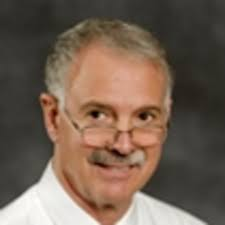
\includegraphics{_images/bob} \end{center}

\hypertarget{hero-2}{%
\subsection{Hero 2}\label{hero-2}}

\begin{center}
\includegraphics{_images/wilma} \end{center}

\hypertarget{workflow-summary}{%
\chapter{Workflow Summary}\label{workflow-summary}}

\hypertarget{r-engine-and-rstudio-ide}{%
\section{R (engine) and Rstudio (IDE)}\label{r-engine-and-rstudio-ide}}

\begin{center}
\includegraphics{_images/rstudio} \end{center}

\hypertarget{rmarkdown}{%
\section{RMarkdown}\label{rmarkdown}}

\begin{center}
\includegraphics{_images/rmarkdown} \end{center}

\hypertarget{bookdown-package}{%
\section{bookdown package}\label{bookdown-package}}

\begin{center}
\includegraphics{_images/bookdown} \end{center}

\hypertarget{github}{%
\section{github}\label{github}}

\begin{center}
\includegraphics{_images/github} \end{center}

\hypertarget{netlify}{%
\section{netlify}\label{netlify}}

\begin{center}
\includegraphics{_images/netlify} \end{center}

\hypertarget{lab-3-coronavirus-visualization-data-wrangling-and-dates}{%
\chapter{\texorpdfstring{Lab 3: \texttt{coronavirus} visualization, data wrangling, and dates}{Lab 3: coronavirus visualization, data wrangling, and dates}}\label{lab-3-coronavirus-visualization-data-wrangling-and-dates}}

\hypertarget{overview}{%
\section{Overview}\label{overview}}

The package is available on GitHub \href{https://github.com/RamiKrispin/coronavirus}{here} and is updated daily.

I use the \texttt{coronavirus} package and use the \texttt{coronavirus::update\_data()} function to keep the data current. This also has the dates preformatted which can be nice.

\hypertarget{lets-look-like-applied-analytics-superstars-and-make-some-neat-visuals.}{%
\section{Let's look like Applied Analytics Superstars and make some neat visuals.}\label{lets-look-like-applied-analytics-superstars-and-make-some-neat-visuals.}}

\begin{Shaded}
\begin{Highlighting}[]
\NormalTok{coronavirus}\SpecialCharTok{::}\FunctionTok{update\_dataset}\NormalTok{()}
\CommentTok{\#\textgreater{} Rows: 633609 Columns: 15}
\CommentTok{\#\textgreater{} {-}{-} Column specification {-}{-}{-}{-}{-}{-}{-}{-}{-}{-}{-}{-}{-}{-}{-}{-}{-}{-}{-}{-}{-}{-}{-}{-}{-}{-}{-}{-}{-}{-}{-}{-}{-}{-}{-}{-}}
\CommentTok{\#\textgreater{} Delimiter: ","}
\CommentTok{\#\textgreater{} chr  (8): province, country, type, iso2, iso3, combined\_...}
\CommentTok{\#\textgreater{} dbl  (6): lat, long, cases, uid, code3, population}
\CommentTok{\#\textgreater{} date (1): date}
\CommentTok{\#\textgreater{} }
\CommentTok{\#\textgreater{} i Use \textasciigrave{}spec()\textasciigrave{} to retrieve the full column specification for this data.}
\CommentTok{\#\textgreater{} i Specify the column types or set \textasciigrave{}show\_col\_types = FALSE\textasciigrave{} to quiet this message.}
\CommentTok{\#\textgreater{} No updates are available}
\end{Highlighting}
\end{Shaded}

\begin{Shaded}
\begin{Highlighting}[]
\FunctionTok{library}\NormalTok{(coronavirus)}
\FunctionTok{library}\NormalTok{(dplyr)}
\FunctionTok{library}\NormalTok{(ggplot2)}
\end{Highlighting}
\end{Shaded}

I'd recommend you always start by trying to understand a bit about the data.

\begin{Shaded}
\begin{Highlighting}[]
\FunctionTok{head}\NormalTok{(coronavirus)}
\CommentTok{\#\textgreater{}         date province country     lat      long      type}
\CommentTok{\#\textgreater{} 1 2020{-}01{-}22  Alberta  Canada 53.9333 {-}116.5765 confirmed}
\CommentTok{\#\textgreater{} 2 2020{-}01{-}23  Alberta  Canada 53.9333 {-}116.5765 confirmed}
\CommentTok{\#\textgreater{} 3 2020{-}01{-}24  Alberta  Canada 53.9333 {-}116.5765 confirmed}
\CommentTok{\#\textgreater{} 4 2020{-}01{-}25  Alberta  Canada 53.9333 {-}116.5765 confirmed}
\CommentTok{\#\textgreater{} 5 2020{-}01{-}26  Alberta  Canada 53.9333 {-}116.5765 confirmed}
\CommentTok{\#\textgreater{} 6 2020{-}01{-}27  Alberta  Canada 53.9333 {-}116.5765 confirmed}
\CommentTok{\#\textgreater{}   cases   uid iso2 iso3 code3    combined\_key population}
\CommentTok{\#\textgreater{} 1     0 12401   CA  CAN   124 Alberta, Canada    4413146}
\CommentTok{\#\textgreater{} 2     0 12401   CA  CAN   124 Alberta, Canada    4413146}
\CommentTok{\#\textgreater{} 3     0 12401   CA  CAN   124 Alberta, Canada    4413146}
\CommentTok{\#\textgreater{} 4     0 12401   CA  CAN   124 Alberta, Canada    4413146}
\CommentTok{\#\textgreater{} 5     0 12401   CA  CAN   124 Alberta, Canada    4413146}
\CommentTok{\#\textgreater{} 6     0 12401   CA  CAN   124 Alberta, Canada    4413146}
\CommentTok{\#\textgreater{}   continent\_name continent\_code}
\CommentTok{\#\textgreater{} 1  North America             NA}
\CommentTok{\#\textgreater{} 2  North America             NA}
\CommentTok{\#\textgreater{} 3  North America             NA}
\CommentTok{\#\textgreater{} 4  North America             NA}
\CommentTok{\#\textgreater{} 5  North America             NA}
\CommentTok{\#\textgreater{} 6  North America             NA}
\end{Highlighting}
\end{Shaded}

For example, what does this summary let us know?

\begin{Shaded}
\begin{Highlighting}[]
\FunctionTok{summary}\NormalTok{(coronavirus}\SpecialCharTok{$}\NormalTok{cases)}
\CommentTok{\#\textgreater{}      Min.   1st Qu.    Median      Mean   3rd Qu.      Max. }
\CommentTok{\#\textgreater{} {-}30974748         0         0       669        29   1368563}
\end{Highlighting}
\end{Shaded}

\begin{enumerate}
\def\labelenumi{\arabic{enumi}.}
\tightlist
\item
  Can you create a visual showing the cases over time for Russia, Spain, US, and Venezuela?
  Also, why might \texttt{filter(cases\ \textgreater{}=\ 0)} be worth using?
\end{enumerate}

\includegraphics{105-coronavirus_lab_files/figure-latex/unnamed-chunk-4-1.pdf}

\begin{enumerate}
\def\labelenumi{\arabic{enumi}.}
\setcounter{enumi}{1}
\tightlist
\item
  Can you show deaths over time for Russia, Spain, US, and Venezuela? And can you play with your geoms and make something neat?
\end{enumerate}

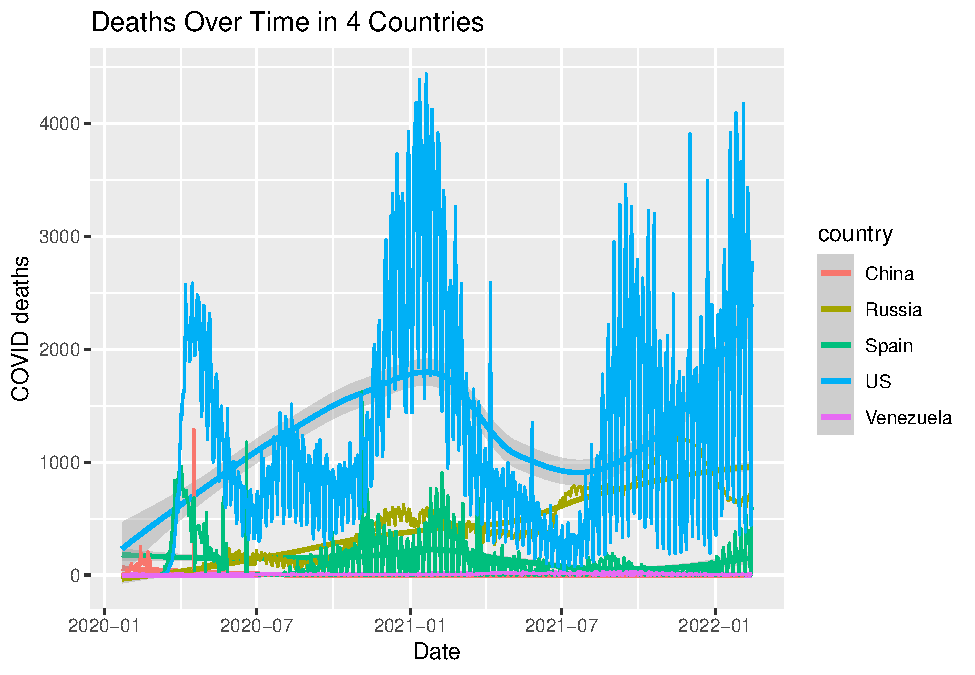
\includegraphics{105-coronavirus_lab_files/figure-latex/unnamed-chunk-5-1.pdf}

\begin{enumerate}
\def\labelenumi{\arabic{enumi}.}
\setcounter{enumi}{2}
\tightlist
\item
  Now let's do a plot of COVID rate (\# confirmed cases / population). Something like this.
\end{enumerate}

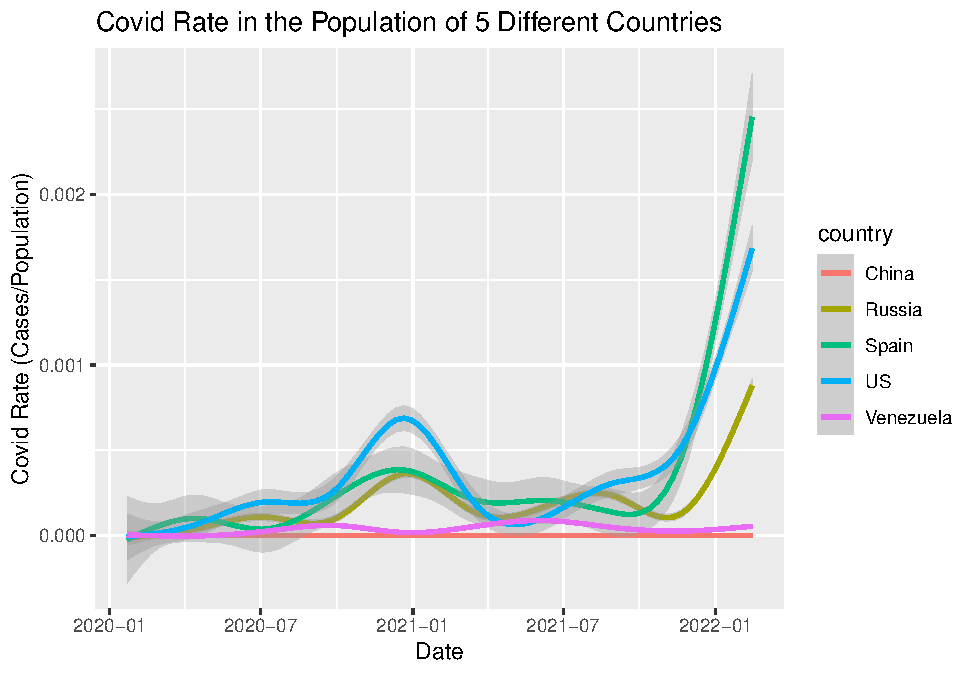
\includegraphics{105-coronavirus_lab_files/figure-latex/unnamed-chunk-6-1.pdf}

\begin{enumerate}
\def\labelenumi{\arabic{enumi}.}
\setcounter{enumi}{3}
\item
  What is and \textbf{is not} useful about the previous illustration?
\item
  Make a chart with cumulative cases. Something like this:
\end{enumerate}

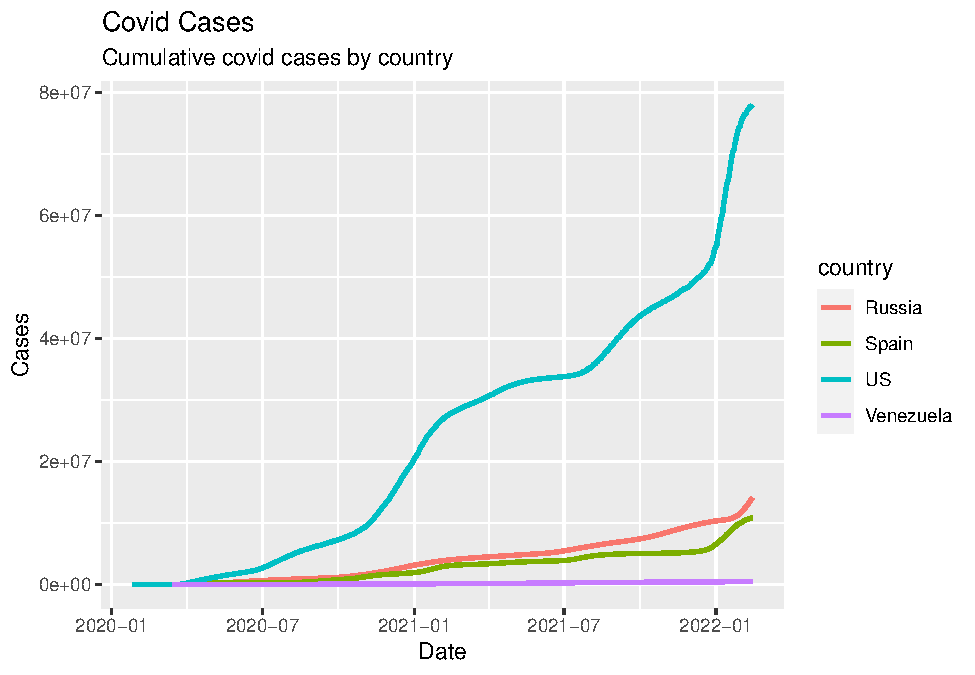
\includegraphics{105-coronavirus_lab_files/figure-latex/unnamed-chunk-7-1.pdf}

\begin{enumerate}
\def\labelenumi{\arabic{enumi}.}
\setcounter{enumi}{5}
\tightlist
\item
  With a little more time and a few extra packages, we \textbf{could} make a graph prettier. Try.
\end{enumerate}

\begin{Shaded}
\begin{Highlighting}[]
\FunctionTok{library}\NormalTok{(scales)}
\FunctionTok{library}\NormalTok{(ggrepel)}
\FunctionTok{library}\NormalTok{(glue)}
\FunctionTok{library}\NormalTok{(lubridate)}
\end{Highlighting}
\end{Shaded}

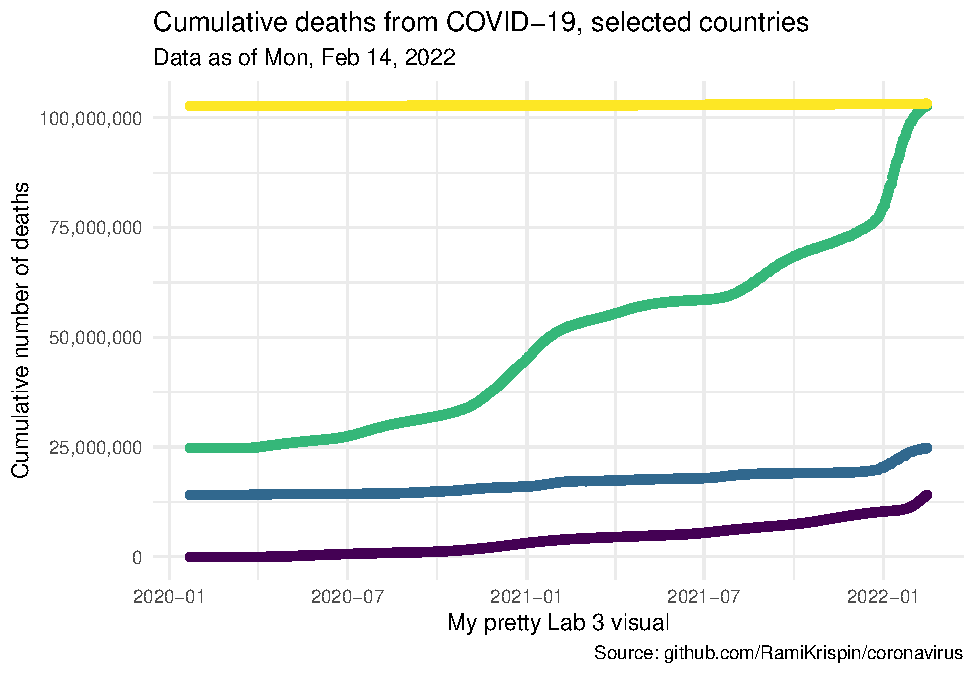
\includegraphics{105-coronavirus_lab_files/figure-latex/unnamed-chunk-9-1.pdf}

\begin{enumerate}
\def\labelenumi{\arabic{enumi}.}
\setcounter{enumi}{6}
\tightlist
\item
  Now let's \textbf{really} have some fun. Let's illustrate death rates relative to confirmed cases. Why is this more challenging than anything we've done so far in this lab? We're going to have to make this data \textbf{tidy}.
\end{enumerate}

One way to play this game.

Let's make a little table of just date, country, and deaths (with a meaningful variable name), and then count observations by coutry just to make sure eveything looks nice.

\begin{verbatim}
#>         date country deaths
#> 1 2020-01-22  Russia      0
#> 2 2020-01-23  Russia      0
#> 3 2020-01-24  Russia      0
#> 4 2020-01-25  Russia      0
#> 5 2020-01-26  Russia      0
#> 6 2020-01-27  Russia      0
#>     country   n
#> 1    Russia 757
#> 2     Spain 754
#> 3        US 757
#> 4 Venezuela 756
\end{verbatim}

Let's make a little table of just confirmed cases.

\begin{verbatim}
#>         date country confirmed
#> 1 2020-01-22  Russia         0
#> 2 2020-01-23  Russia         0
#> 3 2020-01-24  Russia         0
#> 4 2020-01-25  Russia         0
#> 5 2020-01-26  Russia         0
#> 6 2020-01-27  Russia         0
#>     country   n
#> 1    Russia 757
#> 2     Spain 757
#> 3        US 757
#> 4 Venezuela 757
\end{verbatim}

Let's join these together. I use \texttt{left\_join}.

\begin{verbatim}
#>         date country deaths confirmed
#> 1 2020-01-22  Russia      0         0
#> 2 2020-01-23  Russia      0         0
#> 3 2020-01-24  Russia      0         0
#> 4 2020-01-25  Russia      0         0
#> 5 2020-01-26  Russia      0         0
#> 6 2020-01-27  Russia      0         0
#>     country   n
#> 1    Russia 757
#> 2     Spain 757
#> 3        US 757
#> 4 Venezuela 757
\end{verbatim}

Let's add some cumulative statistics as well.

\begin{verbatim}
#>         date country deaths confirmed cumulative_cases
#> 1 2020-01-22  Russia      0         0                0
#> 2 2020-01-23  Russia      0         0                0
#> 3 2020-01-24  Russia      0         0                0
#> 4 2020-01-25  Russia      0         0                0
#> 5 2020-01-26  Russia      0         0                0
#> 6 2020-01-27  Russia      0         0                0
#>   cumulative_deaths rate
#> 1                 0    0
#> 2                 0    0
#> 3                 0    0
#> 4                 0    0
#> 5                 0    0
#> 6                 0    0
\end{verbatim}

Now we can plot some more fun stuff.

\begin{Shaded}
\begin{Highlighting}[]

\FunctionTok{ggplot}\NormalTok{(}\AttributeTok{data =}\NormalTok{ df3,}
       \AttributeTok{mapping =} \FunctionTok{aes}\NormalTok{(}\AttributeTok{x =}\NormalTok{ date,}
                     \AttributeTok{y =}\NormalTok{ rate,}
                     \AttributeTok{color =}\NormalTok{ country)) }\SpecialCharTok{+}
  \FunctionTok{geom\_line}\NormalTok{()}
\end{Highlighting}
\end{Shaded}

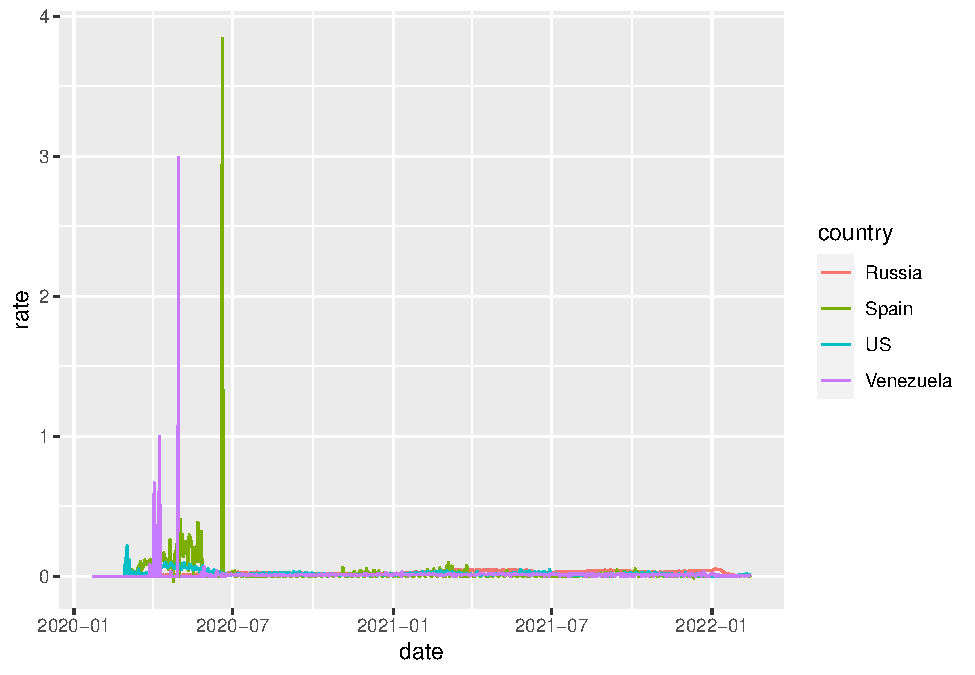
\includegraphics{105-coronavirus_lab_files/figure-latex/unnamed-chunk-15-1.pdf}

\begin{Shaded}
\begin{Highlighting}[]

\FunctionTok{summary}\NormalTok{(df3)}
\CommentTok{\#\textgreater{}       date              country              deaths      }
\CommentTok{\#\textgreater{}  Min.   :2020{-}01{-}22   Length:3028        Min.   :   0.0  }
\CommentTok{\#\textgreater{}  1st Qu.:2020{-}07{-}29   Class :character   1st Qu.:   5.0  }
\CommentTok{\#\textgreater{}  Median :2021{-}02{-}03   Mode  :character   Median : 126.0  }
\CommentTok{\#\textgreater{}  Mean   :2021{-}02{-}03                      Mean   : 452.7  }
\CommentTok{\#\textgreater{}  3rd Qu.:2021{-}08{-}11                      3rd Qu.: 639.2  }
\CommentTok{\#\textgreater{}  Max.   :2022{-}02{-}16                      Max.   :4442.0  }
\CommentTok{\#\textgreater{}                                          NA\textquotesingle{}s   :4       }
\CommentTok{\#\textgreater{}    confirmed         cumulative\_cases    cumulative\_deaths}
\CommentTok{\#\textgreater{}  Min.   : {-}74937.0   Min.   :        0   Min.   :     0   }
\CommentTok{\#\textgreater{}  1st Qu.:    461.5   1st Qu.: 14445698   1st Qu.: 16977   }
\CommentTok{\#\textgreater{}  Median :   7814.0   Median : 25190092   Median : 99431   }
\CommentTok{\#\textgreater{}  Mean   :  34303.5   Mean   : 43523860   Mean   :135068   }
\CommentTok{\#\textgreater{}  3rd Qu.:  28170.0   3rd Qu.:103362932   3rd Qu.:248203   }
\CommentTok{\#\textgreater{}  Max.   :1368563.0   Max.   :103870974   Max.   :364273   }
\CommentTok{\#\textgreater{}                                          NA\textquotesingle{}s   :2147     }
\CommentTok{\#\textgreater{}       rate          }
\CommentTok{\#\textgreater{}  Min.   :{-}0.036576  }
\CommentTok{\#\textgreater{}  1st Qu.: 0.004568  }
\CommentTok{\#\textgreater{}  Median : 0.012750  }
\CommentTok{\#\textgreater{}  Mean   : 0.021680  }
\CommentTok{\#\textgreater{}  3rd Qu.: 0.023227  }
\CommentTok{\#\textgreater{}  Max.   : 3.840391  }
\CommentTok{\#\textgreater{}  NA\textquotesingle{}s   :4}
\FunctionTok{library}\NormalTok{(scales)}
\FunctionTok{library}\NormalTok{(ggrepel)}
\FunctionTok{library}\NormalTok{(glue)}
\FunctionTok{library}\NormalTok{(lubridate)}
\NormalTok{as\_of\_date }\OtherTok{\textless{}{-}}\NormalTok{ df3 }\SpecialCharTok{\%\textgreater{}\%} 
  \FunctionTok{summarise}\NormalTok{(}\FunctionTok{max}\NormalTok{(date)) }\SpecialCharTok{\%\textgreater{}\%} 
  \FunctionTok{pull}\NormalTok{()}
\NormalTok{as\_of\_date\_formatted }\OtherTok{\textless{}{-}} \FunctionTok{glue}\NormalTok{(}\StringTok{"\{wday(as\_of\_date, label = TRUE)\}, \{month(as\_of\_date, label = TRUE)\} \{day(as\_of\_date)\}, \{year(as\_of\_date)\}"}\NormalTok{)}

\FunctionTok{ggplot}\NormalTok{(}\AttributeTok{data =}\NormalTok{ df3,}
       \AttributeTok{mapping =} \FunctionTok{aes}\NormalTok{(}\AttributeTok{x =}\NormalTok{ date, }
                     \AttributeTok{y =}\NormalTok{ cumulative\_cases, }
                     \AttributeTok{color =}\NormalTok{ country)) }\SpecialCharTok{+}
  \CommentTok{\# represent cumulative cases with lines}
  \FunctionTok{geom\_line}\NormalTok{(}\AttributeTok{size =} \FloatTok{0.7}\NormalTok{, }\AttributeTok{alpha =} \FloatTok{0.8}\NormalTok{) }\SpecialCharTok{+}
  \CommentTok{\# add points to line endings}
  \FunctionTok{geom\_point}\NormalTok{() }\SpecialCharTok{+}
  \CommentTok{\# add country labels, nudged above the lines}
  \CommentTok{\# geom\_label\_repel(nudge\_y = 1, direction = "y", hjust = 1) + }
  \CommentTok{\# turn off legend}
  \FunctionTok{guides}\NormalTok{(}\AttributeTok{color =} \ConstantTok{FALSE}\NormalTok{) }\SpecialCharTok{+}
  \CommentTok{\# use pretty colors}
  \FunctionTok{scale\_color\_viridis\_d}\NormalTok{() }\SpecialCharTok{+}
  \CommentTok{\# better formatting for y{-}axis}
  \FunctionTok{scale\_y\_continuous}\NormalTok{(}\AttributeTok{labels =} \FunctionTok{label\_comma}\NormalTok{()) }\SpecialCharTok{+}
  \CommentTok{\# use minimal theme}
  \FunctionTok{theme\_minimal}\NormalTok{() }\SpecialCharTok{+}
  \CommentTok{\# customize labels}
  \FunctionTok{labs}\NormalTok{(}
    \AttributeTok{x =} \StringTok{"My pretty Lab 3 visual"}\NormalTok{,}
    \AttributeTok{y =} \StringTok{"Cumulative number of deaths"}\NormalTok{,}
    \AttributeTok{title =} \StringTok{"Cumulative deaths from COVID{-}19, selected countries"}\NormalTok{,}
    \AttributeTok{subtitle =} \FunctionTok{glue}\NormalTok{(}\StringTok{"Data as of"}\NormalTok{, as\_of\_date\_formatted, }\AttributeTok{.sep =} \StringTok{" "}\NormalTok{),}
    \AttributeTok{caption =} \StringTok{"Source: github.com/RamiKrispin/coronavirus"}
\NormalTok{  )}
\end{Highlighting}
\end{Shaded}

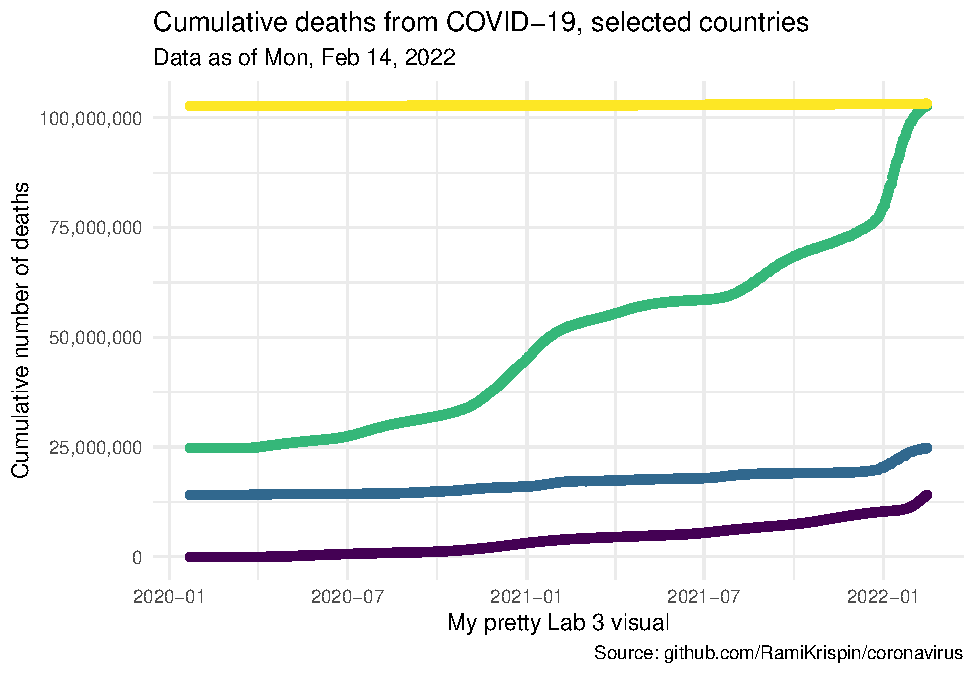
\includegraphics{105-coronavirus_lab_files/figure-latex/unnamed-chunk-15-2.pdf}

\hypertarget{thoughts-questions-discussion}{%
\chapter{Thoughts? Questions? Discussion?}\label{thoughts-questions-discussion}}

\hypertarget{thank-you-for-your-time}{%
\section{Thank you for your time!}\label{thank-you-for-your-time}}

  \bibliography{book.bib,packages.bib}

\end{document}
